\subsection{可用信息：波段差异与光学参数缺口}
\label{sec:optical-inputs}

要判断哪些光谱变化能够进入后续测厚，先要确认全谱是否共享同一把尺度。

标准差衡量一段光谱内反射率围绕平均值的起伏大小。附件1的 $500$--$1000\ \mathrm{cm}^{-1}$ 波段反射率散布标准差约为 $28.9$ 个百分点。
% src:交接/数据档案.json:文件档案.0.工作表.0.分波段描述.1.左闭右开波数区间;文件档案.0.工作表.0.分波段描述.1.反射率统计.样本标准差

相较于低波数段，同一附件的 $3000$--$3500\ \mathrm{cm}^{-1}$ 波段标准差仅约为 $0.189$ 个百分点。这表明原始反射率的散布随波段明显变化，因此在相同窗口比较两角光谱；这里的标准差同时包含趋势与条纹，不用作测量噪声估计。图~\ref{fig:band-spread} 将四条光谱的分波段分布并置后，这一判断落在各段的整体形态上，而不是某一个孤立极值上。
% src:交接/数据档案.json:文件档案.0.工作表.0.分波段描述.1.反射率统计.样本标准差;文件档案.0.工作表.0.分波段描述.6.左闭右开波数区间;文件档案.0.工作表.0.分波段描述.6.反射率统计.样本标准差
% src:交接/图注素材_1.json:3.论文引用建议

\begin{figure}[H]
    \centering
    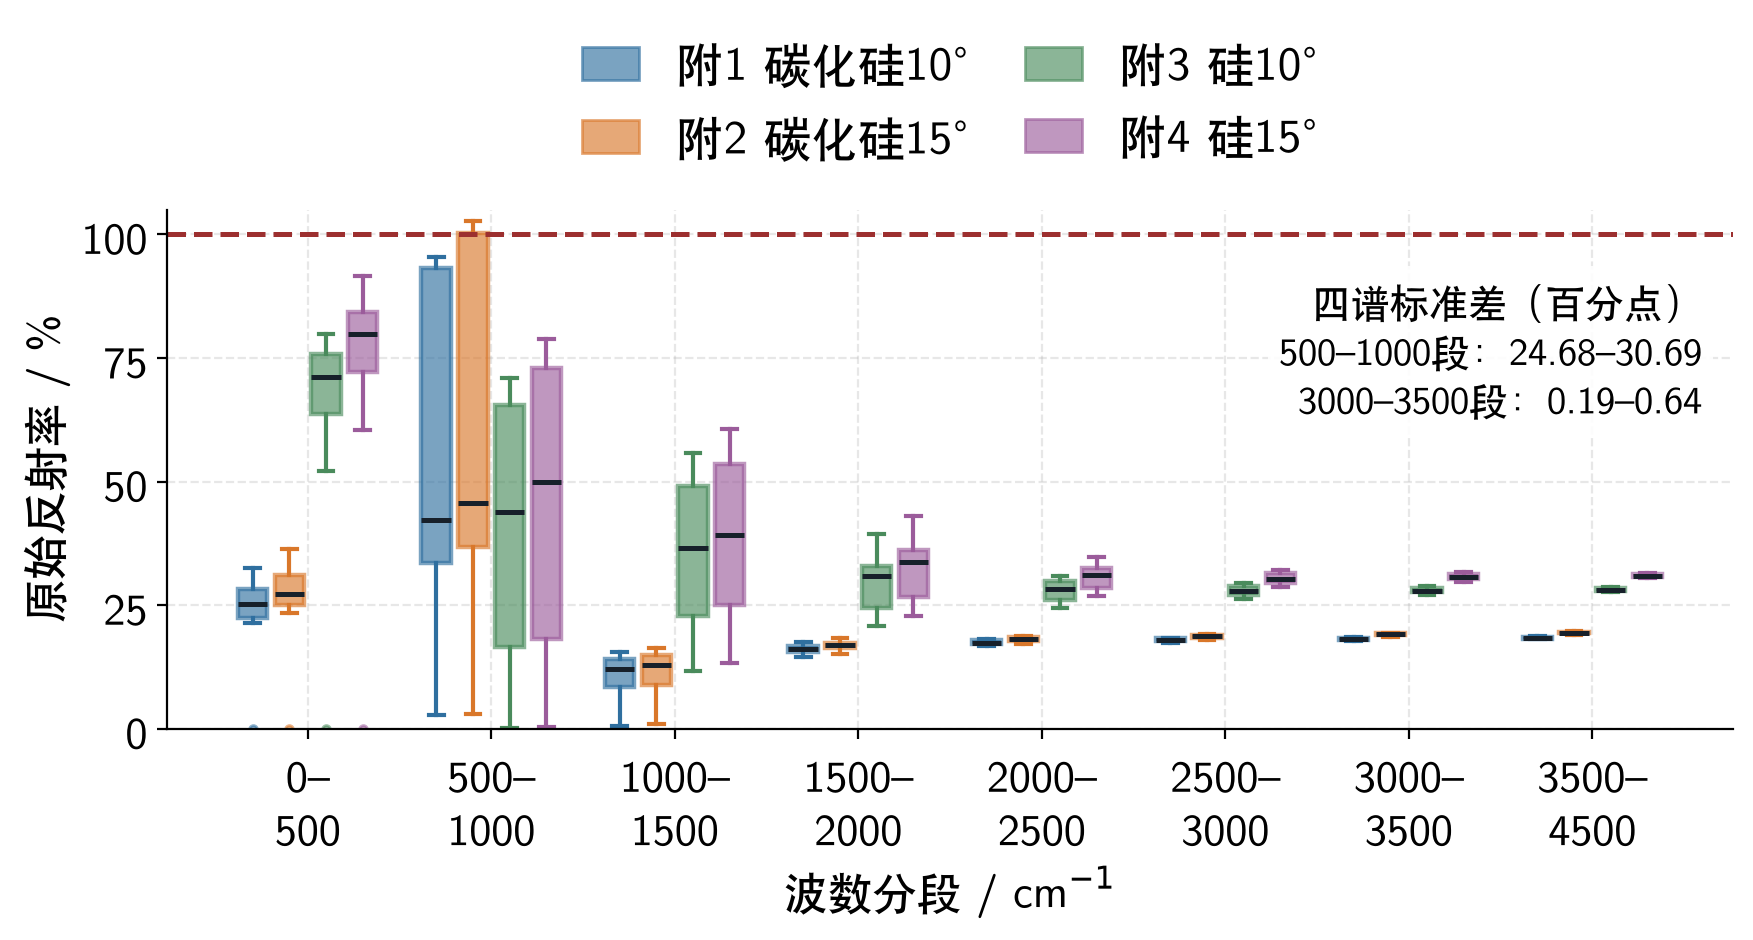
\includegraphics[width=0.96\textwidth]{../求解/公共/图片/波段散布差异不等于噪声.png}
    \caption{四谱低波数段反射率散布更大}
    \label{fig:band-spread}
\end{figure}

这种分段差异决定了选窗还须核对条纹连续性，并通过后文的窗口重估检查其影响。表~\ref{tab:available-info} 对照附件的材料与角度关系，原值保留规则沿用上一节。
% src:交接/数据档案.json:跨文件关系.同片分组;未随附件提供的建模输入

\begin{longtable}{>{\centering\arraybackslash}p{0.22\textwidth} >{\centering\arraybackslash}p{0.22\textwidth} >{\centering\arraybackslash}p{0.22\textwidth} >{\centering\arraybackslash}p{0.22\textwidth}}
\caption{附件与可用光学信息}\label{tab:available-info}\\
\hline
对象 & 材料与角度 & 原始规模与单位 & 标记或缺口\\
\hline
\endfirsthead
\hline
对象 & 材料与角度 & 原始规模与单位 & 标记或缺口\\
\hline
\endhead
附件1 & 碳化硅，$10^\circ$ & $7469$点；\(\mathrm{cm}^{-1}\)、\% & 超百值 $0$\\
附件2 & 碳化硅，$15^\circ$ & $7469$点；\(\mathrm{cm}^{-1}\)、\% & 超百值 $262$\\
附件3 & 硅，$10^\circ$ & $7469$点；\(\mathrm{cm}^{-1}\)、\% & 超百值 $0$\\
附件4 & 硅，$15^\circ$ & $7469$点；\(\mathrm{cm}^{-1}\)、\% & 超百值 $0$\\
共同缺口 & 两种材料，双角观测 & 仅有反射率与波数 & 五类输入缺失\\
\hline
\end{longtable}
% src:交接/数据档案.json:总览.四文件共有波数点数;总览.每块晶圆入射角度;跨文件关系.同片分组;文件档案.0.工作表.0.反射率检查.超过百分之百点数;文件档案.1.工作表.0.反射率检查.超过百分之百点数;文件档案.2.工作表.0.反射率检查.超过百分之百点数;文件档案.3.工作表.0.反射率检查.超过百分之百点数;未随附件提供的建模输入

坐标使用规则见第\ref{sec:common-coordinates}节，测厚还需要附件之外的光学信息。折射率曲线、消光系数、偏振状态、仪器分辨率和真实厚度均未给定；相干长度与光束空间重叠也缺少独立观测。前几项决定相位和反射强度如何换算为厚度，后两项关系到多次返回能否形成可观测干涉。
% src:交接/数据档案.json:未随附件提供的建模输入

初步核对固定折射率的同型峰距法时，上述标定缺口阻断了直接换算，因此将折射率变化显式保留在相位模型中。
% src:交接/实验记录.json:40.尝试;40.现象;40.决定

未标定的光学量将在下一章转为显式假设，并逐项说明其生效位置与检验方法。
